\scanpage{64}\mspage{63}
de $F$, et celles de $A$. De plus, $F$ est somme directe disjointe de ses comp. connexes, i.e. $F=\mathop{\mathrm{Sup}}\limits_i F_i$, les comp. connexes $F_i$ deux à deux disjointes\ldots .

% slanted
\margin{\uline{NB} Dans tout ceci, on n'a pas besoin de $C_3$}

\uline{Composantes connexes de \deleted{$\mathcal F$}la \unsure{contrée|contr.} $\mathcal F$.}

Soit $M=\coprod_{i\in I}M_i$ la décomposition de $M$ en composantes connexes.

Pour toute figure $F$, posons
\[
F_i=\mathop{\mathrm{Sup}}\limits_{X\in M_i\cap M_{\leq F}}X
\]
% slanted
\margin{On appelle $F_i$ la \deleted{\unsure{$F_i$}} $i$-composante de $F$, ou la trace de $F$ sur $M_i$ (ou sur $\mathcal F_i$)}

Alors $F$ est la somme directe des $F_i$, \deleted{et \unsure{?}} Si $F$ est de t.f. \inserted{(ou $I=\pi_0(M)$ fini!)} alors tous les $F_i$ sauf un nb fini \unsure{sont|\deleted{sont}} $\varnothing$.
\margin{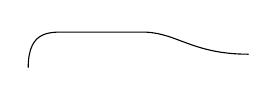
\begin{tikzpicture}[x=1cm,y=1cm]\draw[thin] (0,-.45) .. controls (0,.05) and (.3,0) .. (.55,0) -- (1.5,0) .. controls (1.9,-.02) and (2.1,-.28) .. (2.8,-.28);\end{tikzpicture}}

\deleted{\unsure{Inscrivons|Inversement}} Soit $\mathcal F_i$ l'ens des $F\in\mathcal F$ telle que $\overline F\subset M_i$. Alors \deleted{\unsure{si}} $\mathcal F_i$ satisfait les conditions $C1,C2$\deleted{$,C3$} (et $C3$ aussi, si $\mathcal F$ y satisfait), et $M_i$ est l'ens de ses objets irréductibles.

\deleted{et l'application}
\diagram{\begin{tikzcd}[ampersand replacement=\&,column sep=large,row sep=small,
execute at end picture={\draw[thin,rounded corners=3pt] (oldfamily.south west) -- (oldfigure.west) -- (oldtail.east) .. controls +(right:5pt) and +(right:6pt) .. (oldtail.north east) -- (oldproduct.south west);}]
|[alias=oldfamily]| \mathcal F \arrow[r] \& |[alias=oldproduct]| \prod\mathcal F_i \\
|[alias=oldfigure]| \deleted{F} \arrow[r,mapsto] \& |[alias=oldtail]| \deleted{(F_i)_{i\in I}\ \text{\unsure{ou|où} }F_i\ \text{est le}}
\end{tikzcd}}
Si $F\in\mathcal F$, si $F_i$ sont ses composantes suiv. les $M_i$, alors $\overline{F_i}=\overline F\cap M_i$, $\overline F=\deleted{\coprod}\mathop{\bigcup}\limits_i\overline{F_i}$ (réunion disj)

Pour $i$ fixé, l'application $F\longrightarrow F_i$ commute aux \inserted{Sup quelc., et aux Inf non vides}
\margin{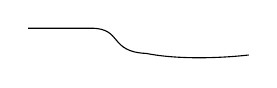
\begin{tikzpicture}[x=1cm,y=1cm]\draw[thin] (0,0) -- (.8,0) .. controls (1.2,0) and (1.02,-.3) .. (1.5,-.32) .. controls (1.9,-.4) and (2.45,-.38) .. (2.8,-.34);\end{tikzpicture}}

L'application
\diagram{\begin{tikzcd}[ampersand replacement=\&,column sep=large]
\mathcal F \arrow[r] \& \prod\mathcal F_i \& F \arrow[r,mapsto] \& (F_i)
\end{tikzcd}}
est injective, et la relation d'ordre de $\mathcal F$ est induite par l'ordre produit
